  Dieses Kapitel behandelt die Analyse von Java Swing Applikationen. Die
  Analyse betrifft die Swing Komponenten, und Komponenten die in einen
  Zusammenhang mit Swing Komponenten stehen. Es werden die gezeigten
  Methoden zur Analyse von Java Swing Applikationen angewendet. Als Ergebniss
  wird eine Kategorisierung der verwendeten Swing Komponenten aufgelistet.
  
  \section{Auswahl der Java Swing Applikationen}
  
  Es sollen drei Applikationen, welche von der Zürcher Kantonalbank entwickelt
  wurden, analysiert werden. Die Applikationen sollen mit Java Swing entwickelt
  worden sein. Die Applikationen werden in der Tabelle
  \ref{tab:zuAnalysierendeJavaSwingApplikationen} aufgelistet.
  \newline
  
  \begin{table}[ht]
    \sffamily 
    \begin{center}
      \begin{tabular}{llp{2cm}p{3.5cm}}
        \toprule
        Applikation & Version & Sourcecode vorhanden & GUI enthält sensible
        Informationen\\
        \midrule
        Strukti Live & Version 1.2 & Ja & Nein\\
        Strukti Online & Version 2.10.0 & Ja & Ja\\
        tbd & ?? & ??\\
        \bottomrule
      \end{tabular}
      \caption{Zu analysierende Java Swing Applikationen}
      \label{tab:zuAnalysierendeJavaSwingApplikationen}
    \end{center}
  \end{table}
  
  \subsection{Begründung}
  
  \begin{description}
  \item[Strukti Live]
  Strukti Live 1.2 wurde gewählt, weil es eine Applikation ist, die
  von der ZKB veröffentlicht wurde. Somit werden bei der Anlayse keine
  sensiblen Informationen preisgegeben.
  \item[Strukti Online]
  Strukti Online 2.10.0 wurde gewählt, weil eine mögliche Migration
  zur Web Applikation schon einmal in der \ac{ZKB} zur Disskusion stant.
  \item[tbd]
  \end{description}
  
  \section{Durchführung der Analyse}
  
  Die Wahl des Verfahrens zur Analyse von Java Swing Applikationen, soll, wie im
  Kapitel \ref{chapter:MethodenZurAnalyseVonJavaSwingApplikationen} erläutert,
  gemacht werden. Gemäss des gewählten Verfahrens sollen alle Komponenten, die
  Java Swing zur Verfügung stellt, in der Applikation gesucht werden. Die
  Komponenten können in der Dokumentation von Oracle\footnote{Oracle ist die
  Firma, welche Java entwickelt.} zu Java Swing gefunden werden, siehe
  \cite{SwingComponentsByOracle}. Zudem sollen alle Komponenten, welche durch
  externe Bibliotheken zur Verfügung gestellt werden, gesucht werden. Die Suche
  findet durch einen visuellen Vergleich der Komponenten statt, wenn möglich
  kann auch der Sourcecode in die Suche miteinbezogen werden. Um das ganze für
  den Leser nachvollziehbar zu machen, sollen die gefundenen Komponenten mit
  Hilfe von Screenshots gezeigt werden, wenn die Applikation für die
  Öffentlichkeit bestimmt ist. Falls es sich bei der Analyse um eine
  Applikation für den internen Gebrauch handelt, werden keine Screenshots
  gezeigt. Es könnten Rückschlüsse auf die Business-Logik gemacht werden, was
  nicht im Sinne der \ac{ZKB} ist.
  
  Als Resultat soll eine Auflistung aller gefundenen Komponenten erstellt
  werden. Die Auflistung wird in folgende Gruppen unterteilt:
  
  \begin{itemize}
    \item Top-Level-Komponenten
    \item Intermediate-Komponenten
    \item Atomic-Komponenten
    \item Spezielle Komponenten
  \end{itemize}
  
  \noindent
  Als Ergänzung zu den Komponenten, sollen auch erkannte GUI Paradigmen
  aufgelistet werden. Dabei gibt es Design-Patterns, siehe
  \cite{DesignPattern}, die verwendet werden. Zusätzlich können durch das
  Zusammenspiel einzelner Swing Komponenten auch ``neue'' Komponenten entstehen.
  Leider sind die meisten Design-Pattern und ``neuen'' Komponenten nicht mehr
  mit Hilfe von Screenshots nachvollziehbar. Das jeweilige Verhalten soll
  desshalb in ein paar Sätzen beschrieben werden.
  
  Als Resultat soll eine Auflistung erstellt werden. Die Auflistung wird in die
  folgenden Gruppen unterteilt:
  
  \begin{itemize}
    \item Design-Patterns
    \item neue Komponenten
  \end{itemize}
  
  \section{Strukti Live}
  
  Strukti Live ist ein Lerntool der Zürcher Kantonalbank für strukturierte
  Produkte. Die Applikation kann auf dem Internetauftritt \footnote{Unter der
  Internetadresse \url{http://www.zkb.ch/struktilive} sind alle nötigen
  Informationen zu Strukti Live enthalten.} der \ac{ZKB} heruntergeladen
  werden. Es wurde die aktuelle Version 1.2 für die Analyse verwendet.
  
  In der Tabelle \ref{tab:bibliothekenStruktiLive} sind alle verwendeten
  Bibliotheken, welche eine Interaktion mit dem \ac{GUI} haben, ersichtlich.
  \newline
  
  \begin{table}[ht]
    \sffamily 
    \begin{center}
      \begin{tabular}{lp{4.5cm}ccp{2cm}}
        \toprule
        Bibliothek & Funktion & Version & Lizenz & Quellcode vorhanden?\\
        \midrule
        core-renderer.jar & XHtml und CSS Renderer für Swing & R8 & LGPL & Ja\\
        %bogatyr\_0.60.jar & Abstraktion einiger Swing Komponenten & 0.60 & GPL
        %& Ja\\
        jfreechart-1.0.10.jar & Charting Library für Java & 1.0.10 & LGPL & Ja\\
        %jcommon-1.0.13.jar & JFreeChart extension & 1.0.13 & LGPL & Ja\\
        %ZKB\_CICD\_0.40.jar & Swing Komponenten im ZKB Design & 0.40 & - & Ja\\
        \bottomrule
      \end{tabular}
      \caption{Verwendete Bibliotheken von Strukti Live 1.2}
      \label{tab:bibliothekenStruktiLive}
    \end{center}
  \end{table}
  
  \subsection{Gefundene Komponenten}
  
  \subsubsection{Top-Level-Komponenten}
  
  \begin{itemize}
    \item \(javax.swing.JDialog\), siehe Abbildung \ref{img:SL-02}
    \item \(javax.swing.JFrame\) mit \(javax.swing.JRootPane\), siehe Abbildung
    \ref{img:SL-01}
  \end{itemize}
  
  \subsubsection{Intermediate-Komponenten}
  
  \begin{itemize}
    \item \(javax.swing.JPanel\), siehe Abbildung \ref{img:SL-01}
    \item \(javax.swing.JScrollPane\), siehe Abbildung \ref{img:SL-01}
    \item \(javax.swing.JTabbedPane\), siehe Abbildung \ref{img:SL-03}
  \end{itemize}
  
  \subsubsection{Atomic-Komponenten}
  
  \begin{itemize}
    \item \(javax.swing.JButton\), siehe Abbildung \ref{img:SL-01}
    \item \(javax.swing.JCheckBox\), siehe Abbildung \ref{img:SL-01}
    \item \(javax.swing.JLabel\), siehe Abbildung \ref{img:SL-01}
    \item \(javax.swing.JRadioButton\), siehe Abbildung \ref{img:SL-02}
    \item \(javax.swing.JSlider\), siehe Abbildung \ref{img:SL-02}
    \item \(javax.swing.JTextField\), siehe Abbildung \ref{img:SL-02}
    \item \(javax.swing.JToolTip\), siehe Abbildung \ref{img:SL-03}
  \end{itemize}
  
  \subsubsection{Spezielle Komponenten}
  
  \begin{itemize}
    \item \(javax.swing.JLabel\) als externer Link, siehe Abbildung
    \ref{img:SL-03}
    \item \(org.jfree.chart.JFreeChart\), siehe Abbildung \ref{img:SL-02}
    \item \(org.xhtmlrenderer.simple.XHTMLPanel\), siehe Abbildung
    \ref{img:SL-03}
  \end{itemize}
  
  \begin{figure}[htb]
    \begin{center}
      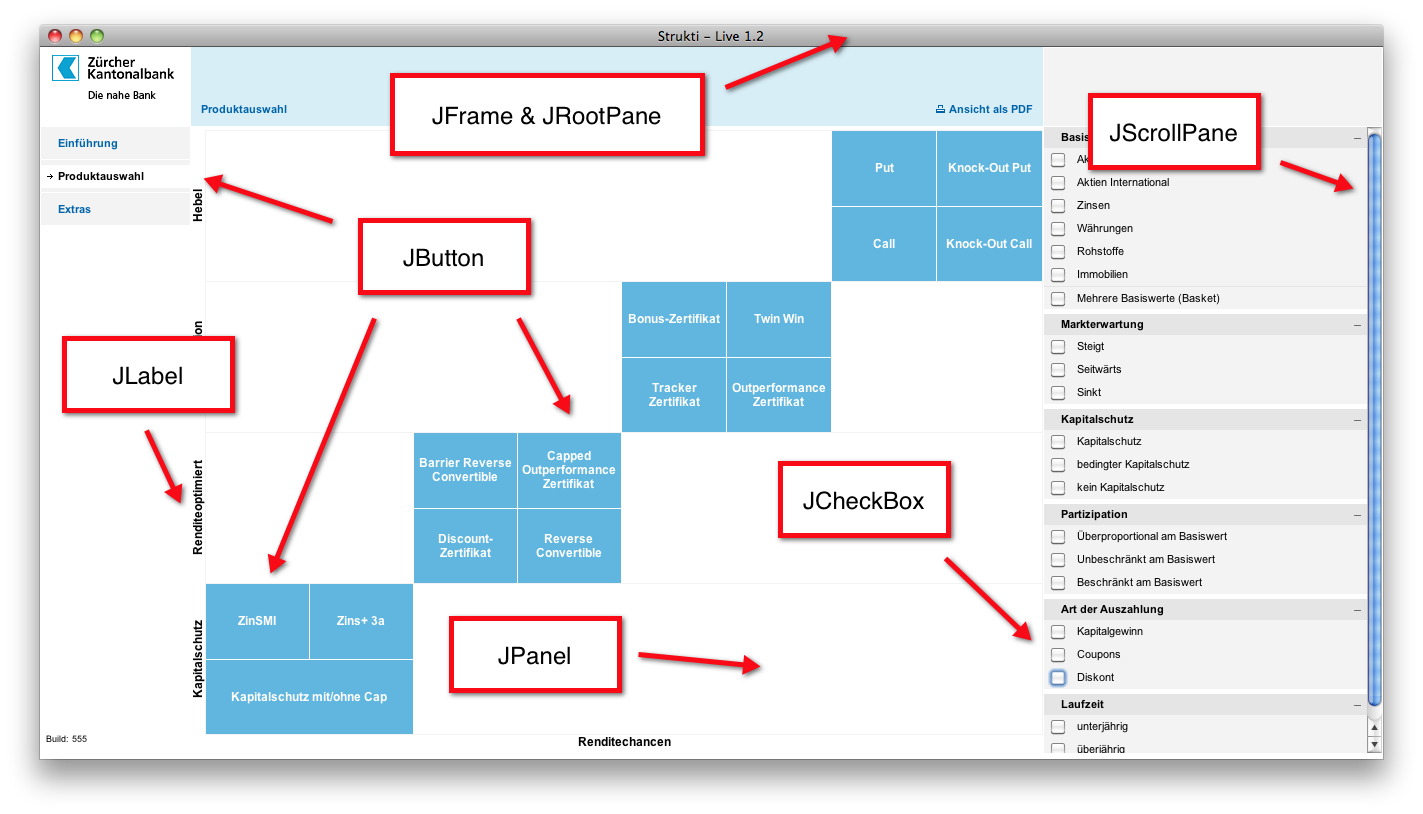
\includegraphics[width=\textwidth]{./image/SL/SL-01.png}
      \caption{Strukti Live 1.2 - Screenshot I}
      \label{img:SL-01}
    \end{center}
  \end{figure}
  
  \begin{figure}[htb]
    \begin{center}
      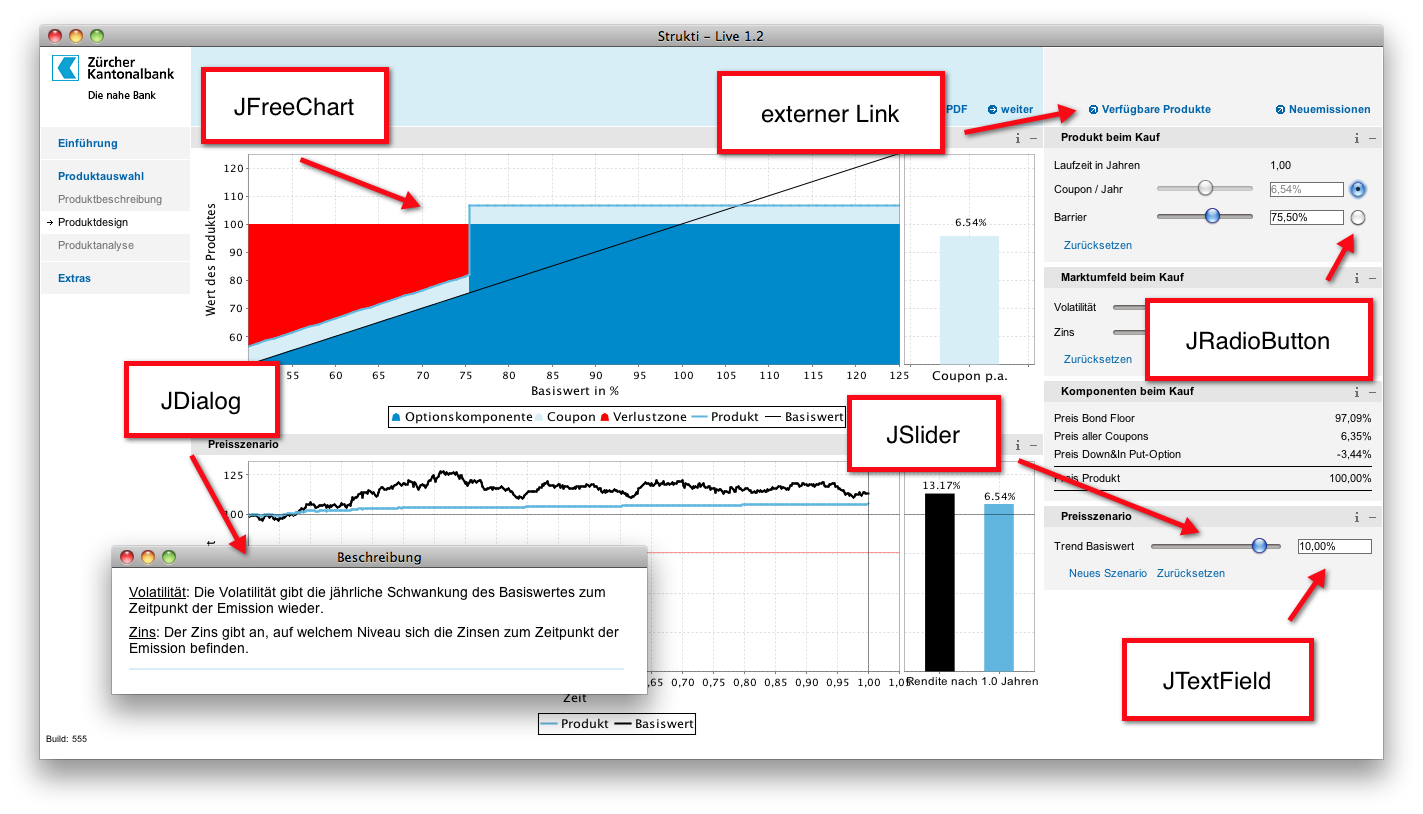
\includegraphics[width=\textwidth]{./image/SL/SL-02.png}
      \caption{Strukti Live 1.2 - Screenshot II}
      \label{img:SL-02}
    \end{center}
  \end{figure}
  
  \begin{figure}[htb]
    \begin{center}
      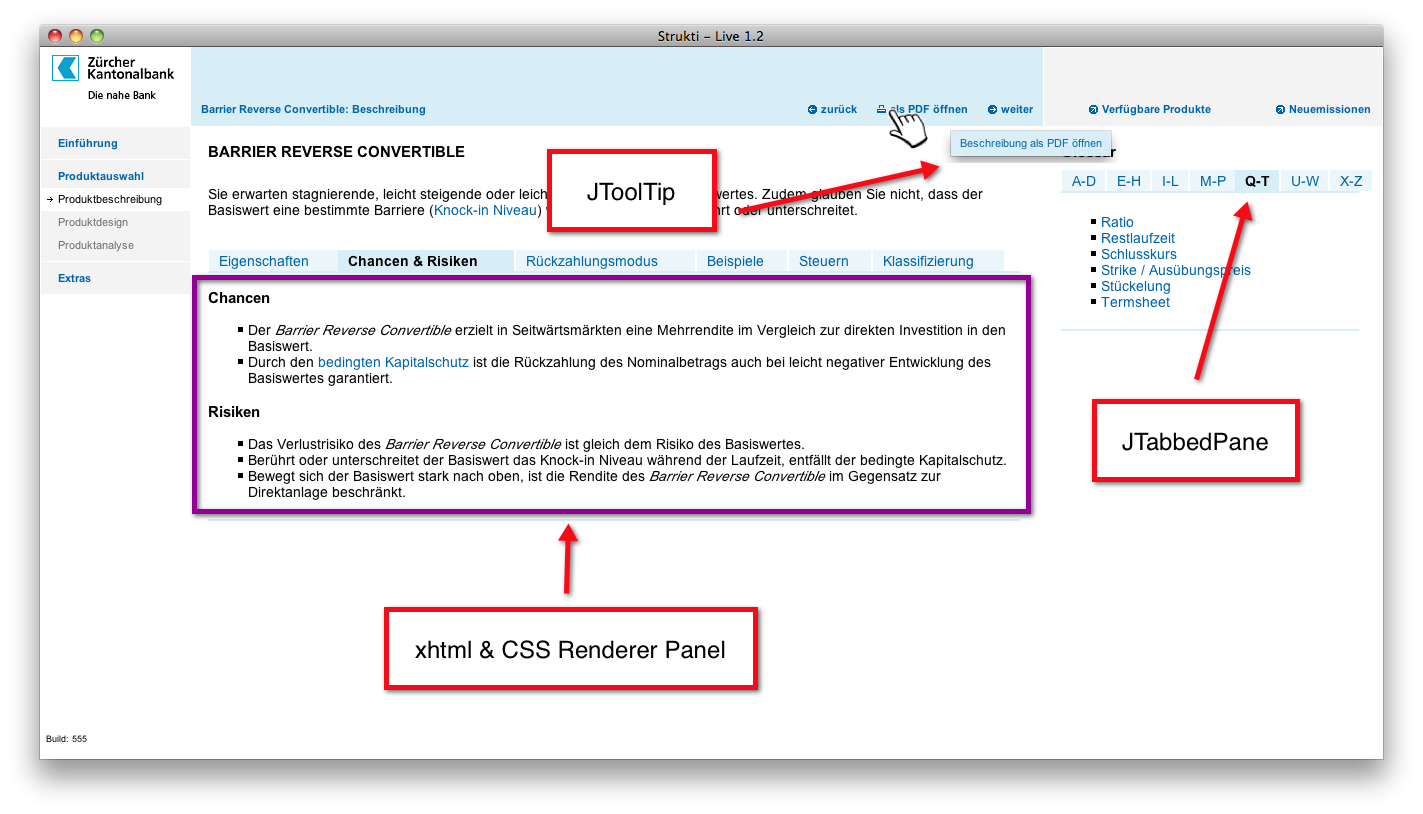
\includegraphics[width=\textwidth]{./image/SL/SL-03.png}
      \caption{Strukti Live 1.2 - Screenshot III}
      \label{img:SL-03}
    \end{center}
  \end{figure}
  
  \subsection{Gefundene Design-Patterns}
  
  \begin{description}
    \item[Menüführung]
    Die Menüführung wurde durch das Observer-Pattern, siehe
    \cite{ObserverDesignPattern}, implementiert. Dabei wird in einem Modell
    der jeweilige Status der Applikation durch das Drücken eines
    \(javax.swing.JButton\) angepasst, wobei sich die jeweiligen
    \(javax.swing.JPanel\), welche auf Änderungen des Modells höhren, sich neu
    zeichnen.
    \item[Komponentenupdate]
    Ebenfalls mit dem Observer-Pattern, siehe \cite{ObserverDesignPattern},
    wurde die Aktualisierung von Komponenten, welche zusammen hängen,
    realisiert. Als Beispiel dient ein Verbund der Komponenten
    \(javax.swing.JTextField\), \(javax.swing.JSlider\) und
    \(org.jfree.chart.JFreeChart\). Dabei werden bei einer Änderung des Wert bei
    dem Slider oder dem Textfeld die Werte aller anderen Komponenten
    entsprechend aktualisiert.
  \end{description}
  
  \subsection{Gefundene ``neue'' Komponenten}
  
  \begin{description}
    \item[Button-Matrix]
    JButtons werden in einer Matrix angeordnet, um sie entsprechend ihrer
    Funktion zu ordnen. Hinter jedem JButton steckt ein Finanzprodukt, das bei
    einem Klick angezeigt werden kann. Die JButtons können entsprechend
    ihrer Renditechancen (x-Achse) und deren Kapitalschutzes (y-Achse)
    angeordnet werden.
    \item[Akkordeon]
    Ein Verbund von \(javax.swing.JPanel\) Komponenten, bei welchem ein
    Panel als Titelleiste funktioniert. In der Titelleiste kann über ein Minus-
    oder Plussymbol ein weiterer Panel ein- oder ausgeklappt werden. Zudem gibt
    es in der Titelleiste ein Info-Button, wo ein Dialog mit
    Hintergrundinformationen geöffnet werden kann.
  \end{description}
  
  \section{Strukti Online}
  
  Strukti Online ist ein Emissionstool der \ac{ZKB} für strukturierte Produkte.
  Die Applikation wird aktuell nur zum internen Gebrauch entwickelt und basiert
  auf Java Swing. Es wurde die aktuelle Version 2.10.0 für die Analyse
  verwendet.
  
  Da es sich um eine interne Applikation handelt, werden keine Screenshots
  der Applikation gezeigt, da anhand dessen eventuell Rückschlüsse auf die
  Business-Logik gemacht werden könnte.
  
  In der Tabelle \ref{tab:bibliothekenStruktiOnline} sind alle verwendeten
  Bibliotheken, welche eine Interaktion mit dem \ac{GUI} haben, ersichtlich,
  und ob deren Sourcecode zugänglich ist.
  
  \begin{table}[ht]
    \sffamily 
    \begin{center}
      \begin{threeparttable}
        \begin{tabular}{lp{4.5cm}ccp{2cm}}
          \toprule
          Bibliothek & Funktion & Version & Lizenz & Quellcode vorhanden?\\
          \midrule
          core-renderer.jar & XHtml und CSS Renderer für Swing & R8 & LGPL &
          Ja\\
          jfreechart-1.0.10.jar & Charting Library für Java & 1.0.10 & LGPL
          & Ja\\
          forms.jar & Layout System aus der JGoodies Palette & 1.2.1 &
          BSD\tnote{1} & Ja\\
          swingx-1.0.jar & Swing Komponenten Erweiterung & 1.0 & LGPL & Ja\\
          \bottomrule
        \end{tabular}
        \caption{Verwendete Bibliotheken von Strukti Online 2.10.0}
        \label{tab:bibliothekenStruktiOnline}
        \begin{tablenotes}[++]\footnotesize 
          \item[1] Es handelt sich dabei um die ``BSD open source license''
        \end{tablenotes} 
      \end{threeparttable}
    \end{center}
  \end{table}
  
  \subsection{Gefundene Komponenten}
  
  \subsubsection{Top-Level-Komponenten}
  
  \begin{itemize}
    \item \(javax.swing.JDialog\)
    \item \(javax.swing.JFrame\) mit \(javax.swing.JRootPane\)
  \end{itemize}
  
  \subsubsection{Intermediate-Komponenten}
  
  \begin{itemize}
    \item \(javax.swing.JLayerdPane\)
    \item \(javax.swing.JPanel\)
    \item \(javax.swing.JScrollPane\)
    \item \(javax.swing.JTabbedPane\)
  \end{itemize}
  
  \subsubsection{Atomic-Komponenten}
  \begin{itemize}
    \item \(javax.swing.JButton\)
    \item \(javax.swing.JCheckbox\)
    \item \(javax.swing.JComboBox\)
    \item \(javax.swing.JFileChooser\)
    \item \(javax.swing.JLabel\)
    \item \(javax.swing.JRadioButton\)
    \item \(javax.swing.JPasswordField\)
    \item \(javax.swing.JSeparator\)
    \item \(javax.swing.JSlider\)
    \item \(javax.swing.JSpinner\)
    \item \(javax.swing.JTable\)
    \item \(javax.swing.JTextArea\)
    \item \(javax.swing.JTextField\)
    \item \(javax.swing.JTextPane\)
    \item \(javax.swing.JToolTip\)
  \end{itemize}
  
  \subsubsection{Spezielle Komponenten}
    
  \begin{itemize}
    \item \(javax.swing.JLabel\) als externer Link
    \item \(org.jfree.chart.JFreeChart\)
    \item \(org.xhtmlrenderer.simple.XHTMLPanel\)
    \item \(org.jdesktop.swingx.JXBusyLabel\)
    \item \(org.jdesktop.swingx.JXDatePicker\)
  \end{itemize}
    
  \subsection{Gefundene Design-Patterns}
  
  \begin{description}
    \item[MVC]
    Das Zusammenspiel von Model, View und Kontroller wurde strikte nach dem
    MVC-Design-Pattern implementiert, siehe \cite{GUIDesignPatterns} S. 15ff.
    \item[Observer]
    Einfache Aktuallisierungen zwischen Komponenten wurden strikte nach dem
    Observer-Design-Pattern implementiert, siehe \cite{GUIDesignPatterns} S.
    2ff.
    \item[Tabellen-Filter]
    Durch die Verwendung von JRadioButton, JComboBox, JXDatePicker und JSpinner
    wurden bei den meisten Ansicht von Tabellen Filter gebaut, damit die Daten
    auf das Wesentliche reduziert werden können. Datei wurde für jede relevante
    Spalten der Tabelle entsprechend deren Datentyp eine dieser Komponenten
    gewählt.
  \end{description}
  
  \subsection{Gefundene ``neue'' Komponenten}
  
  \begin{description}
    \item[Button-Matrix]
    JButtons werden in einer Matrix angeordnet, um sie entsprechend ihrer
    Funktion zu ordnen. Hinter jedem JButton steckt ein spezifisches
    vorbewertetes Finanzprodukt, das bei einem Click angezeigt werden kann.
    Die JButtons können entsprechend ihrer Laufzeit (x-Achse) und der
    Underlyings\footnote{Auch Basiswerte genannt, siehe \cite{Basiswerte}} des
    hinterlegten Finanzprodukts (y-Achse) angeordnet werden. Die Matrix, kann
    wie eine Tabelle nach Laufzeiten sortiert werden.
    \item[Akkordeon]
    Ein Verbund von \(javax.swing.JPanel\) Komponenten, bei welchem ein
    Panel als Titelleiste funktioniert. In der Titelleiste kann über ein Minus-
    oder Plussymbol ein weiterer Panel ein- oder ausgeklappt werden.
    \item[Zeit-Panel]
    Durch die Kombination einer \(org.jdesktop.swingx.JXDatePicker\) und einer
    \(javax.swing.JSpinner\) Komponente kann ein Datum mit Uhrzeit ausgewählt
    werden.
  \end{description}
  
  \section{tbd}
  
  Tbd ist ein blablabla Tool
  
  In der Tabelle \ref{tab:bibliothekenTbd} sind alle verwendeten
  Bibliotheken, welche eine Interaktion mit dem \ac{GUI} haben, ersichtlich,
  und ob deren Sourcecode zugänglich ist.
  
  \begin{table}[ht]
    \sffamily 
    \begin{center}
      \begin{tabular}{lllr}
        \toprule
        Bibliothek & Version & Lizenz & Sourcecode vorhanden \\
        \midrule
        tbd & xx & xx & Ja\\
        tbd & xx & xx & Ja\\
        \bottomrule
      \end{tabular}
      \caption{Verwendete Bibliotheken von TBD X.X}
      \label{tab:bibliothekenTbd}
    \end{center}
  \end{table}
  
  \subsection{Gefundene Komponenten}
  
  \subsubsection{Top-Level-Komponenten}
  
  \begin{itemize}
    \item top
  \end{itemize}
  
  \subsubsection{Intermediate-Komponenten}
  
  \begin{itemize}
    \item intermediate
  \end{itemize}
  
  \subsubsection{Atomic-Komponenten}
  
  \begin{itemize}
    \item atomic
  \end{itemize}
  
  \subsubsection{Spezielle Komponenten}
    
  \begin{itemize}
    \item special
  \end{itemize}
  
  \subsection{Gefundene GUI Paradigmen}
    
  \subsubsection{Design-Patterns}
  
  \begin{description}
    \item[Pattern]
  \end{description}
  
  \subsubsection{``neue'' Komponenten}
  
  \begin{description}
    \item[new Component]
  \end{description}
  
  \section{Liste der Komponenten}
  
  Die Auflistung aller gefundenen Komponenten soll als Grundlage für die Analyse
  der Web Frameworks dienen. Bei der Analyse soll geprüft werden, ob die hier
  erkannten Komponenten implementiert werden können. Folgende Komponenten
  wurden in den Applikationen gefunden:
  
  \subsection{Top-Level-Komponenten}
  
  \begin{itemize}
    \item top
  \end{itemize}
  
  \subsection{Intermediate-Komponenten}
  
  \begin{itemize}
    \item intermediate
  \end{itemize}
  
  \subsection{Atomic-Komponenten}
  
  \begin{itemize}
    \item atomic
  \end{itemize}
  
  \subsection{Spezielle Komponenten}
  
  \begin{itemize}
    \item special
  \end{itemize}
  
  \section{Liste der GUI Paradigmen}
  
  Die Auflistung aller gefundenen GUI Paradigmen soll als Grundlage für die
  Analyse der Web Frameworks dienen. Bei der Analyse soll geprüft werden, ob
  die hier erkannten GUI Paradigmen implementiert werden können. Folgende GUI
  Paradigmen wurden in den Applikationen gefunden:
      
  \subsection{Design-Patterns}
  
  \begin{description}
    \item[Pattern]
  \end{description}
  
  \subsection{``Neue'' Komponenten}
  
  \begin{description}
    \item[new Component]
  \end{description}